%%%%%%%%%%%%%%%%%%%%%%%%%%%%%%%%%%%%%%%%%%%%%%%%%%%%%%%%%%%%%%%%%%%%%%%%%%%%%%%%
%2345678901234567890123456789012345678901234567890123456789012345678901234567890
%        1         2         3         4         5         6         7         8

\documentclass[letterpaper, 10 pt, conference]{ieeeconf}  % Comment this line out
\IEEEoverridecommandlockouts


\usepackage[ngerman]{babel}
\usepackage{paralist, tabularx}
\usepackage{subfigure}
\usepackage{amsmath}

\usepackage{soul}
\usepackage{xcolor}
\newcommand\sichen[1]{\textcolor{red}{sichen: #1}}
\newcommand\siqi[1]{\textcolor{blue}{siqi: #1}}
\title{\LARGE \bf
Data Plane Verification as Program Verification
}


\author{Siqi Liu,
Sichen Song
}

\usepackage[T1]{fontenc}
\usepackage{graphicx}
\usepackage{listings}
\begin{document}



\maketitle
\thispagestyle{empty}
\pagestyle{empty}



\section{INTRODUCTION}
Data plane verification is an emerging field of computer networking, in which the behavior of network data plane is verified to follow a specification. 

To perform data plane verification, the network topology and forwarder configurations are typically encoded into a model, which is checked against the specification. For example, the Header Space Analysis (HSA) encodes the network nodes into functions on packet state, which consists of packet header and packet location~\cite{hsa}. HSA then simulates a symbolic packet being forwarded through the network model to verify reachability and other properties. Anteater, on the other hand, models the network and its specification as SAT formulas on the packet header and reduces the network verification problem into a SAT problem, which can be solved using existing SAT solvers such as Z3~\cite{z3}.

The existing works focuses on verifying stateless network nodes and consequently does not work on networks with stateful load balancers or NAT boxes. Although data plane specification language has been proposed in NoD~\cite{nod} and NetPlumber~\cite{netp}, the languages has limited expressiveness and requires times for network operators to learn. Lastly, the generated model is hard to understand or debug due to extensive use of logical formulas.

To address the above issues, we investigation into modeling the data plane as a computer program and utilizing existing symbolic execution tool, KLEE~\cite{klee}, to verify network properties. In the following sections, we provide the rationale behind reducing network verification into a program verification in \S~\ref{sec:rationale}. We then present the architecture of our verifier that reduce network verification into program verification in \S ~\ref{sec:overall}. We dive into details of code generation in \S~\ref{sec:codegen}. We also propose potential optimizations that could potentially use pre-computation to improve the performance of verification in \S~\ref{sec:opt}. Lastly we discuss the evaluation results in \S~\ref{sec:eval}.


\section{Rationale}\label{sec:rationale}

Symbolic execution for program verification models program input as a set of potential values and explores the control flow graph of the program by executing the program and adding path constrains to the symbolic variables whenever having conditional statements. By keeping track of a set of potential input that leads to certain execution path, feasibility of  execution path can be calculated by checking whether the path conditions is satisfiable. In this way, by exploring all reachable execution paths, the program can be verified.

Symbolic execution is similar to Header Space Analysis(HSA) as they both use equivalence classes of input to ensure efficient and comprehensive exploration a directed graph. Both of them also reason about reachability in the graph by transforming the problem as a satisfiability problem of path condition.

This similarity motivates us to explore the idea of transforming the network verification problem into a program verification problem and transform network reachability and other properties to verify into code reachability. The idea can be implemented by generating the network configuration and verification problem into a network simulator on symbolic packet inputs. This reduction can have the following advantages:

\begin{enumerate}
  \item The generated model is a network simulator written in C++, which is easier to understand and debug compared to logical formula based modeling.
  \item Existing optimizer in compiler such as constant propagation and dead code elimination can operate on the generated code.
  \item Stateful nodes such as NAT can be modeled as a mutable objects that forward packets.
  \item The specification is essentially C++ code operating on packet state or path, which is easier to learn by network operators.
  \item The generated network simulator can be executed with concrete packet input, which can be reused to debug network configurations by visualizing packet forwarding.
\end{enumerate}


\section{Overall Design}\label{sec:overall}
The overall design of our network verification framework is illustrated in fig.~\ref{fig:arch}. 

To reduce data plane verification into program verification, code generation is extensively used. Overall there are three different types of code generators: the network node generator, the topology generator, and verification generator. Network node generator generates forwarders and other nodes in the network from its configurations such as FIBs and ACLs. A variety of node types is supported such as ECMP routers and stateful NAT boxes. Topology generator generates the code that takes a packet state (header, location) as input and move a packet through the network for one step. The packet is first fed into the corresponding forwarder to make a forwarding action. The output packet is then transformed into a input packet of the next hop by looking up the network topology. Lastly, the verification generator will generate the "main function" that injects symbolic packets into the network and keep forwarding it through the network. The most import part of it is the main loop that keeps forwarding packets step by step using the topology generator. Depending on the property to verify, the generator may also record of packet paths and other states for later property checks. The code generators may embed comments in the generated code to facilitate post-processing.

These generated C++ code will be compiled into LLVM intermediate representation (IR) using the LLVM C++ front end Clang++. These IR is then used by KLEE for symbolic execution. KLEE will invoke LLVM optimization passes on the input IR and symbolically execute the program to maximize line coverage and check if it can fail any assertion in the program. The resulting coverage file is then fed into a post processing script to check if the property-to-verify is maintained by the network. The generated comments by code generators acts has hints for the post processor to better understand the coverage and thus make verification decisions.

\sichen{mention the limitations: black box KLEE. One solution.}
\begin{figure}[]
  \centering
  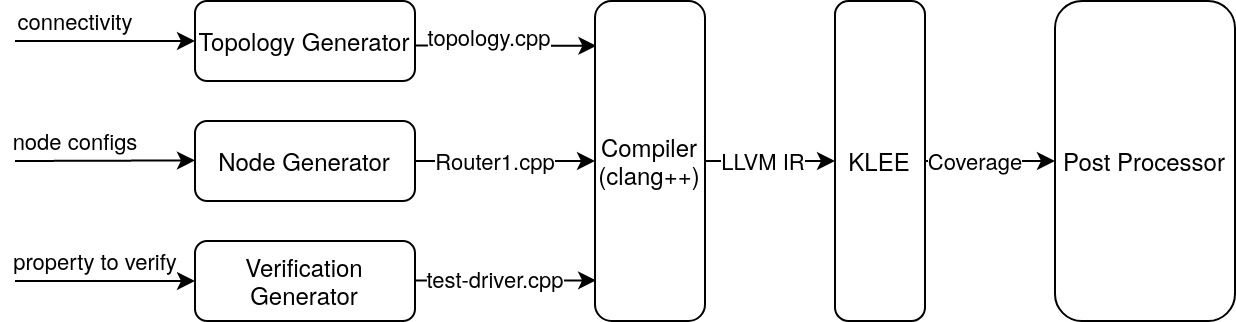
\includegraphics[width=\linewidth]{overview.png}
  \caption{Architecture}
  \label{fig:arch}
\end{figure}

\section{Code Generation}\label{sec:codegen}
Code generator is the primary part of reducing data plane verification into program verification. The generators will generate a  executable C++ program that asserts the property-to-verify with symbolic packet inputs such that symbolic execution can later be used to check these assertions. The code is also annotated with generated comments serving as hints to help the poster processor to translate code coverage report from KLEE into network verification results.
\subsection{Constrains}
Symbolic execution can perform poorly when the program has large loops, requires variable length in-memory data structures, or make many unnecessary branches. Being aware of these limitations, code generator of this framework inlines table (for example, FIB) lookup as a sequence of branches, instead of relying on in-memory data structures. It also bounds all loops to bound the total amount of execution paths. 

\subsection{Packet State}
Inspired by HSA~\cite{hsa}, the packet state is the combination of header and location as shown in listing \ref{code:state}.
\begin{lstlisting}[language=C,caption=Packet State,label=code:state,captionpos=b]
struct Header {
  uint32_t src_address;
  uint32_t dst_address;
...
};

struct PktState {
  Header header;
  int node;
  int port;
};
\end{lstlisting}

\subsection{Stateless Network Routers}
Stateless network Routers are generated based on their FIB and ACL configurations. An C++ class with the node name is generated that has a \emph{forward} method that transforms the input packet state to the output packet state. Listing~\ref{code:stateless-router} shows a generated router class. Note that a linear scan over the routing table from longest prefix to shortest prefix is used for FIB lookup, which may result in poor performance. Optimization of FIB lookup is discussed in sec.~\ref{sec:opt}. Also, the \emph{[reached] Router4} comment act as a hint to facilitate post processing of node reachability.

\begin{lstlisting}[
  language=C,
  caption=Packet State,
  label=code:stateless-router,
  captionpos=b,
  basicstyle=\small]
class Router4 {
  public:
  
  PktState 
  forward(PktState stateIn) { //[reached] Router4
    int node = stateIn.node;
    int portIn = stateIn.port;
    Header &header = stateIn.header;
    int portOut = forwardTable(header.dst_address);
    if (!acl(header, portIn, portOut)) 
        return {header, node, -1};
    return {header, node, portOut};
  }
  
  int forwardTable(uint32_t dst) {
  if ((dst >> 16) == (0xa000000 >> 16))//10.0.0.0/16
    return 1;
  if ((dst >> 16) == (0xa010000 >> 16))//10.1.0.0/16
    return 2;
  return -1;
    ...
  }
  
  bool acl(Header header, int ingress, int egress) {
    if (
    header.dst_port == 80 &&
    header.protocol == 6 &&
    true)
      return false; // DenyHTTP
    ...
    return true; // false as drop
  }
};
\end{lstlisting}


\subsection{Network}

The network with connectivity and node is generated as a C++ class, which instantiates all the nodes and expose a function that takes a packet state and makes one step of packet forwarding. The input packet is first processed by the corresponding forwarder to be transformed to an output packet. Then, by looking up network connectivity, the output packet is moved to the input port of the other end of the link.  Listing~\ref{code:topology} shows a generated network class.

\begin{lstlisting}[  language=C,
  caption=Packet State,
  label=code:topology,
  captionpos=b,
  basicstyle=\small]
class Topology {
  public:
  
  PktState 
  node_execute(PktState pktState) {
    int node = pktState.node;
    Header &header = pktState.header;
    int port = pktState.port;
    if (node == 0) {
      return node0.forward(pktState);
    }
    ...
    
    assert(0); //[node-dispatch-failed]
  }
  
  static PktState 
  link_function(PktState in) {
    int node = in.node;
    int port = in.port;
    Header &header = in.header;
    if (node == 0 && port == 1)
    return {header, 1, 1};
    if (node == 1 && port == 1)
    return {header, 0, 1};
    ...
  }
  
  public:
  Router1 node0;
  Router2 node1;
...
};
\end{lstlisting}

\subsection{Reachability Query Test Driver}
The reachability query test driver simply injects a symbolic packet at the user-selected node and simulate the packet forwarding until the packet exits or TTL runs out. KLEE will enumerate the entire header space trying to cover every line of code, which includes the forward method of each node object. Thus, the coverage report of KLEE can be used to infer if a node is reachable by checking if its corresponding class and method is covered. To cover a reasonable number of packet forwarding while bounding the main loop for packet forwarding, we set the TTL to be two times the diameter of the network topology.
Listing~\ref{code:reachability-driver} shows a generated network class.

\begin{lstlisting}[  language=C,
  caption=Packet State,
  label=code:reachability-driver,
  captionpos=b,
  basicstyle=\small]
class Network : public Topology {
  public:
  void forward(PktState pktState) {
    if (klee_is_replay())
      printf("Starting port: %d %d\n"...);
    for (int hop = 0; hop < 6; hop++) {
      PktState forwardedPktState = 
        node_execute(pktState);
      if (forwardedPktState.port == PORT_DROP) {
        if (klee_is_replay())
          printf("Drop by: %d %d\n"...);
        return;
      }
      pktState = link_function(forwardedPktState);
      if (klee_is_replay())
        printf("Forward to: %d %d => %d %d\n"...);
      if (pktState.port == PORT_DROP) return;
    }
    assert(0); //[TTL-Drop] potential loop
    return;
  }
};

int main() {
  Header header;
  klee_make_symbolic(&header, 
  	sizeof(header), "header");
  
  Network n;
  n.forward(PktState(header,Router1Id,0));
  
  return 0;
}
\end{lstlisting}

\subsection{Loop Detection Query}
Intuitively, loop detection should check if a packet reenters a router. However, to minimize the states and simplify the problem, we detect loop by checking for TTL violations. By settings a TTL much larger than network diameter and checking for TTL drop. Loops can be detected. The loop detection test driver is exactly the same as the reachability query test driver in listing~\ref{code:reachability-driver}. Note that the generated comment \emph{[TTL-Drop] potential loop} is used for post processors to identify the test packet that could trigger loop.
\subsection{Stateful Nodes}

\subsection{Other Queries}

\subsection{Optimization}\label{sec:opt}
\sichen{todo:}

\section{Evaluation}\label{sec:eval}

\section{FUTURE DIRECTION}\label{sec:fd}

\section{CONCLUSIONS}\label{sec:c}




\addtolength{\textheight}{-12cm}  
\bibliographystyle{IEEEtran}
\bibliography{bibs}


\end{document}

